\documentclass[xcolor=table]{beamer}
\usepackage{fontspec}
\usepackage{natbib}
\usepackage{gb4e} 
\usepackage[table]{xcolor}
\usepackage{booktabs} 
%\usepackage{color}
\usepackage{graphicx}
\usepackage{tikz}
\usetikzlibrary{trees}

% \setmainfont[Mapping=tex-text]{Charis SIL}
\let\sfdefault\rmdefault
%\newcommand{\racine}[1]{\begin{math}\sqrt{#1}\end{math}} 
\newfontfamily\phon[Mapping=tex-text,Ligatures=Common,Scale=MatchLowercase,FakeSlant=0.3]{Charis SIL} 
\newcommand{\ipa}[1]{{\phon \mbox{#1}}} %API tjs en italique
\newcommand{\grise}[1]{\cellcolor{lightgray}\textbf{#1}} 
\newcommand{\ra}{$\Sigma_1$} 
\newcommand{\rc}{$\Sigma_3$} 
\newcommand{\ro}{$\Sigma$} 
 \begin{document}

 \title{Grammaticalization pathways based on denominal derivations in Japhug Rgyalrong}
 \author{Guillaume Jacques}
 \maketitle
 
  \begin{frame} 
 \frametitle{Japhug and other Rgyalrongic languages} 
 \begin{figure}[H]
\centering
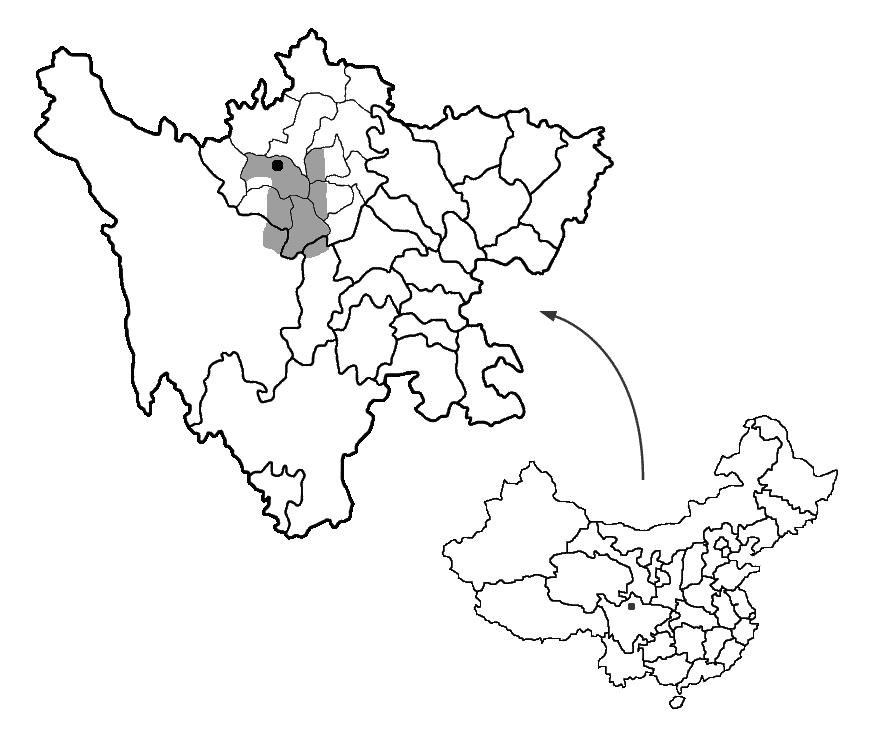
\includegraphics[height=28mm]{carte.JPG}
\end{figure}
 
%Unlike most languages of the Sino-Tibetan family: 
 
 \begin{enumerate}[<+->]
 \item Polysynthetic (polypersonal agreement, incorporation), complex templatic morphology (\citealt{jacques13harmonization})
  \item Direct-inverse agreement system (\citealt{jacques10inverse})
 \item Complex morphophonological alternations
 \item Very rich voice morphology (antipassive, passive, causative, applicative etc)
 \item Complex consonant clusters (for instance \ipa{lɟɣaʁ} `put on')
 \item Strict accusative AND ergative pivots in various domains of the morphosyntax.
 \item Barely any non-trivial morphosyntactic feature in common with Chinese or Burmese.
 \end{enumerate}
  
  \end{frame}   

  \begin{frame} 
 \frametitle{Areal context} 
 \begin{enumerate}[<+->]
 \item Considerable impact of various dialects of Tibetan on the Japhug lexicon.
 \item Tibetan influence on the evidential system
 \item Some linkers are of Tibetan origin (for instance \ipa{nɤ} in the protasis of conditionals).
 \item The ergative \ipa{kɯ} and the genitive \ipa{ɣɯ} have been recently borrowed from Amdo Tibetan.
 \item Some recent lexical influence from Sichuan Chinese.
 \end{enumerate}
  \end{frame}   


  \begin{frame} 
 \frametitle{Grammaticalization in Japhug} 

A considerable part of the rich morphology found in Japhug is relatively recent and its origin still relatively transparent.

 \begin{enumerate}[<+->]
    \item S/A Nominalizing prefix $\Rightarrow$  Generic person marking and 2$\rightarrow$1 portmanteau prefix
   \item second person + passive $\Rightarrow$ 1$\rightarrow$2 portmanteau prefix
   \item causative+passive $\Rightarrow$ progressive
	\item Garden variety changes:
 \begin{enumerate}	
 \item Orientational prefixes $\Rightarrow$  various TAM markers (\citealt{jackson07irrealis, lin11direction, jacques14linking})
 \item Motion verbs $\Rightarrow$ Associated motion (\citealt{jacques13harmonization})
  \item etc...
  \end{enumerate}
 \end{enumerate}

  \end{frame}   

  \begin{frame} 
 \frametitle{Grammaticalization} 
 \begin{itemize}
\item Voice derivations (Antipassive, Applicative, Causative, Passive, Deexperiencer)
\item Incorporation
\item Comitative
\end{itemize}
\end{frame}   

  \begin{frame} 
 \frametitle{Denominal derivations in Japhug} 
  \framesubtitle{List of denominal prefixes in Japhug} 
 
No zero derivation from noun to verb 
 
\begin{tabular}{lllllllll} \toprule
Form& Property \\
\midrule
\ipa{nɯ}--, \ipa{nɤ}-- & intransitive and transitive \\
\ipa{rɯ}--, \ipa{rɤ}-- & intransitive and transitive \\
\ipa{ɣɯ}--, \ipa{ɣɤ}-- & intransitive and transitive \\
\ipa{sɯ}--, \ipa{sɤ}--, \ipa{sɯɣ}--  & transitive verb with instrument\\
&intransitive verb of position \\
\ipa{mɤ}-- & transitive verb with body part\\
& intransitive verb of position \\
\ipa{sɤ}-- & intransitive verb (property) \\
\ipa{a}-- & intransitive verb (shape) \\
\ipa{aɣɯ}-- & intransitive verb (property) \\
    \bottomrule
\end{tabular}

\end{frame}   

  \begin{frame} 
 \frametitle{Voice derivations vs denominal derivations} 
 
\begin{tabular}{lllllllll} \toprule
Form& Voice & Corresponding denominal prefix \\
\midrule
\ipa{rɤ}-- & Antipassive &    \ipa{rɤ}-- (intransitive dynamic verbs)\\
\ipa{nɯ}-- & Applicative &    \ipa{nɯ}-- (transitive dynamic verbs)\\
\ipa{sɯ}-- & Causative &    \ipa{sɯ}-- (instrumental transitive verb )\\
\ipa{a}-- & Agentless Passive &    \ipa{a}-- (stative verb )\\
\ipa{sɤ}--  & Deexperiencer &    \ipa{sɤ}-- (stative verb expressing a property)\\
    \bottomrule
\end{tabular}

\end{frame}   

\begin{frame} 
\frametitle{Voice derivations vs denominal derivations} 
\framesubtitle{Antipassive} 

From \citet{jacques14antipassive}

\begin{tabular}{lllllllll} \toprule
\multicolumn{2}{c}{basic  transitive verb}  & \multicolumn{2}{c}{derived  intransitive verb}  \\
\midrule
\ipa{roʁ}   &	to carve &  	\ipa{rɤ-roʁ}   &	to carve things \\  
\ipa{tɕɤβ}   &	to burn &  	\ipa{rɤ-tɕɤβ}   &	to burn land \\  
\ipa{ɕpʰɤt}   &	to patch &  	\ipa{rɤ-ɕpʰɤt}   &	to patch things \\  
\ipa{pɣaʁ}   &	to turn over &  	\ipa{rɤ-pɣaʁ}   &	to reclaim land \\  
\ipa{tʂɯβ}   &	to sew &  	\ipa{rɤ-tʂɯβ}   &	 to sew things \\   
\ipa{ɕar}   &	to search &  	\ipa{rɤ-ɕar}   &	to search for things \\ 
\ipa{ŋa}   &	to owe  (specific quantity)&  	\ipa{rɤ-nŋa}   &	to owe money \\  
\ipa{ntsɣe}   &	to sell &  	\ipa{rɤ-tsɣe}   &	to sell things \\  
\ipa{χtɯ}   &	to buy &  	\ipa{ra-χtɯ}   &	to buy things \\  
\bottomrule
\end{tabular}
\end{frame}   

\begin{frame} 
\frametitle{Voice derivations vs denominal derivations} 
\framesubtitle{Antipassive} 
  \begin{exe}
\ex
\gll \ipa{tɤ-rʑaβ} 	\ipa{nɯ} 	\ipa{pjɤ-rɤ-ɕpʰɤt}   \\
    \textsc{indef.poss}-wife \textsc{top} \textsc{ifr-antipass:non.human}-mend \\
 \glt    `The wife mended (clothes).' (The raven 19)
\end{exe} 
 
   \begin{exe}
\ex
\gll \ipa{tɤ-rʑaβ} 	\ipa{nɯ} 	\ipa{kɯ}	\ipa{pjɤ-ɕpʰɤt}   \\
    \textsc{indef.poss}-wife \textsc{dem} \textsc{erg} \textsc{ifr}-mend \\
 \glt    `The wife mended it.' 
\end{exe} 

\end{frame}   
 
\begin{frame} 
\frametitle{Voice derivations vs denominal derivations} 
\framesubtitle{Antipassive} 
Denominal in \ipa{rɯ--}/\ipa{rɤ--}
\begin{tabular}{llllll}
\toprule
 Derived verb& Meaning &Base noun  & Meaning \\
\midrule
  \ipa{rɤ-ŋgɯm} & to lay an egg & \ipa{(tɤ)-ŋgɯm} &egg \\
  \ipa{rɯ-ɕmi} & to speak & \ipa{(tɯ)-ɕmi} & word  \\
  \ipa{rɯ-kʰɤjxwi} & to have a meeting (it) & \ipa{kʰɤjxwi} & meeting \\
 \bottomrule
\end{tabular}
\end{frame}    
 
 \begin{frame} 
\frametitle{Voice derivations vs denominal derivations} 
\framesubtitle{Antipassive} 
 
Bare action nominal (or patient nominal): bare verb root (+possessive prefix)
 \begin{enumerate}
\item Transitive verb $\rightarrow$ bare action nominal (\ipa{ɕpʰɤt} `to patch (vt)' $\rightarrow$ \ipa{(tɤ)-ɕpʰɤt} `patch (n)')
\item bare action nominal $\rightarrow$ intransitive denominal verb \ipa{rɤ-ɕpʰɤt} `to patch clothes' (= do patching')
\end{enumerate}
 
\end{frame}    
 
  \begin{frame} 
\frametitle{Voice derivations vs denominal derivations} 
\framesubtitle{Antipassive} 
 
Common irregularities between the base noun and the antipassive verb:
\begin{itemize}
\item
  \begin{enumerate}
\item Transitive verb \ipa{pɣaʁ} `turn over (including fields)' 
 \item Antipassive verb \ipa{rɤ-pɣaʁ} `reclaim land' 
  \item Action nominal \ipa{tɯ-pɣaʁ} `land reclamation' 
\end{enumerate}
 \item
   \begin{enumerate}
\item Transitive verb \ipa{ŋa} `owe (a certain amount a of money)' 
 \item Antipassive verb \ipa{rɤ-nŋa} `owe money' 
  \item Action nominal \ipa{(tɯ)-nŋa} `debt' 
\end{enumerate}
\end{itemize}

\end{frame}    
 
 \begin{frame} 
\frametitle{Voice derivations vs denominal derivations} 
\framesubtitle{Applicative} 
 
 \begin{tabular}{lllllllll} \toprule
basic verb  & &derived  verb &\\
\midrule
 \ipa{aʑɯʑu}  & wrestle	& \ipa{nɤʑɯʑu}  & wrestle with\\
\ipa{akhu}  &	shout, call&\ipa{nɤkhu}  & shout at \\
\ipa{akhɤzŋga}&	shout, call&\ipa{nɤkhɤzŋga}  & shout at \\
\ipa{andzɯt}  &	bark&\ipa{nɤndzɯt}  & bark at \\
\ipa{amdzɯ}  &sit & \ipa{nɤmdzɯ}  &look after\\
\ipa{aɣro}&play&\ipa{nɤɣro} & play with \\
    \ipa{stu}  &believe (vi)	& \ipa{nɤstu}  & believe (vt)\\
\midrule
\ipa{mbɣom}  &	be hurried & \ipa{nɯmbɣom}  & look  forward to\\
&&& miss s.o.\\
\ipa{ŋke}  &go on foot	& \ipa{nɯŋke}  & look for \\
\ipa{rga}  &	like, be glad (vi) & \ipa{nɯrga}  &like (vt) \\
\ipa{sŋom}  &	envy (vi) & \ipa{nɯsŋom}  &envy (vt) \\
\midrule
  \ipa{bɯɣ}  &miss (vi)	& \ipa{nɯɣbɯɣ}  & miss (vt)\\
  \ipa{mu} & be afraid & \ipa{nɯɣmu} & be afraid of \\
\bottomrule
\end{tabular}
\end{frame}    

 \begin{frame} 
\frametitle{Voice derivations vs denominal derivations} 
\framesubtitle{Applicative} 
\begin{tabular}{lllllllll} \toprule
Base noun& Meaning & Derived verb & Meaning & \\
\midrule
\ipa{mbɯrlɤn} &plane & \ipa{nɯ-mbɯrlɤn} &to plane    &vt\\
\ipa{smɤn} &medicine & \ipa{nɯ-smɤn} &to treat    &vt\\
\ipa{mkɤɣɯr} &necklace & \ipa{nɯ-mkɤɣɯr} &to wear as a necklace    &vt\\
\ipa{ʁgra} & enemy& \ipa{nɯ-ʁgra} & to treat as an enemy&vt\\
\ipa{(tɯ)-skʰrɯ} &body  & \ipa{nɯ-skʰrɯ} &to be pregnant with &vt\\
\ipa{kʰɤjxwi} & meeting&  \ipa{nɯ-kʰɤjxwi} & to have a meeting (about sth) & vt  \\
    \bottomrule
\end{tabular}
\end{frame}    
 
  \begin{frame} 
\frametitle{Voice derivations vs denominal derivations} 
\framesubtitle{Causative} 
 
 
\begin{tabular}{lllllllll} \toprule
 transitivity & base & & derived & \\
 \midrule
 intr. & \ipa{ɕe} & go & \ipa{sɯɣ-ɕe} & send \\
  tr. & \ipa{ɕɯm} & brood & \ipa{sɯ-ɕɯm} & cause to brood \\
  intr. & \ipa{ndzur} & stand & \ipa{sɯɣ-ndzur} & cause to stand up \\
  tr. & \ipa{ndza} & eat & \ipa{sɯ-ndza} & cause to eat \\ 
    intr. & \ipa{tso} & understand & \ipa{sɯɣ-tso} & cause to understand \\
  tr. & \ipa{tsɯm} & take away & \ipa{sɯ-tsɯm} &  send \\ 
 \bottomrule
\end{tabular}

\end{frame}    
 
   \begin{frame} 
\frametitle{Voice derivations vs denominal derivations} 
\framesubtitle{Causative} 
 
 
\begin{tabular}{llllll}
\toprule
  Derived verb& Meaning &Base noun  & Meaning \\
\midrule
\ipa{sɤ-kʰɯ} & to smoke& \ipa{(tɤ)-kʰɯ} & smoke\\
 \ipa{sɯ-fsaŋ} & to perform  & \ipa{fsaŋ} & fumigation \\
&ritual fumigation\\
\ipa{sɯɣ-tsʰaʁ} & to sieve & \ipa{tsʰaʁ} & sieve\\
\ipa{sɯɣ-tsʰwi} & to dye & \ipa{tsʰwi} & colour, paint\\
 \ipa{sɯ-ɕtʂi}& to cause to sweat & \ipa{(tɯ)-ɕtʂi} & sweat\\
 \ipa{sɤ-rmi} & to give a name & \ipa{(tɤ)-rmi} & name\\
\bottomrule
\end{tabular}
\end{frame}  

   \begin{frame} 
\frametitle{Voice derivations vs denominal derivations} 
\framesubtitle{Deexperiencer} 

Experiencer $\rightarrow$ Stimulus

\begin{tabular}{llllll}
\toprule
  Derived verb& Meaning &Base verb  & Meaning \\
\midrule
 \ipa{sɤ-scit} & to be nice & \ipa{scit} & be happy \\
 \ipa{sɤ-ɕke} & to be burning & \ipa{ɕke} & be burned \\
 \ipa{sɤ-ŋgio} & to be slippery & \ipa{ŋgio} & slip \\
 \ipa{sɤ-rga} & to be lovely & \ipa{rga} & like \\
\bottomrule
\end{tabular}
\end{frame}    

   \begin{frame} 
\frametitle{Voice derivations vs denominal derivations} 
\framesubtitle{Deexperiencer} 
\begin{tabular}{llllll}
\toprule
  Derived verb& Meaning &Base noun  & Meaning \\
\midrule
 \ipa{sɤ-ndɤɣ} & to be poisonous & \ipa{(tɤ)-ndɤɣ} & poison \\
 \ipa{sɤ-mbrɯ} & to be angry & \ipa{(tɤ)-mbrɯ} & anger \\
\bottomrule
\end{tabular}
\end{frame}    

   \begin{frame} 
\frametitle{Voice derivations vs denominal derivations} 
\framesubtitle{Summary}
\begin{exe}
\ex
\glt \textsc{action nominalization} of transitive verb + \textsc{intransitive denominal derivation} $\Rightarrow$ \textsc{antipassive}
\ex
\glt \textsc{action nominalization} of intransitive verb + \textsc{transitive denominal derivation} $\Rightarrow$ \textsc{applicative} / \textsc{causative}
\end{exe}


Parallels in West Mande (\citealt{creissels12antip}) and Eskaleut (\citealt{fortescue96halftrans}) 
 \end{frame}    
 
    \begin{frame} 
\frametitle{Incorporation vs denominal derivations} 

 \citet{jacques12incorp}
 
   \begin{exe}
\ex
\begin{xlist}[(ii)]
\exi{(i)} 
\gll     \ipa{cɯ-pʰɯt} \ipa{nɯ-βzu-t-a}  \\
  stone-clearing \textsc{pfv}-do-\textsc{pst-1sg} \\
\exi{(ii)} 
\gll     \ipa{nɯ-ɣɯ-cɯ-pʰɯt-a}  \\
  \textsc{pfv}-\textsc{derivation}-stone-take.out-\textsc{1sg} \\
\exi{(iii)} 
\gll     \ipa{cɯ} \ipa{nɯ-pʰɯt-a}  \\
  stone \textsc{pfv}-take.out-\textsc{1sg} \\
  \end{xlist}
 \glt   I cleared the stones (from the field). (elicitation, Chen Zhen)
 
\end{exe}   
 
 
\end{frame}    
 
    \begin{frame} 
\frametitle{Incorporation vs denominal derivations} 
\framesubtitle{Noun + Verb synthetic compounds} 

\begin{itemize}
\item
\begin{enumerate}
\item \ipa{cʰa} `alcohol' + \ipa{tsʰi} `drink (vt)' $\Rightarrow$  \ipa{cʰɤ-tsʰi} ``alcohol drinking''
\item \ipa{cʰɤ-tsʰi} ``alcohol drinking'' + denominal prefix $\Rightarrow$  \ipa{ɣɯ-\textbf{cʰɤ}-tsʰi } ``drink alcohol''
\end{enumerate}
\item
\begin{enumerate}
\item \ipa{pɕawtsɯ} `money' (from Chinese) + \ipa{fsoʁ} `accumulate (vt)' (from Tibetan) $\Rightarrow$   \ipa{pɕawtsɯ-fsoʁ} ``money earning''
\item \ipa{pɕawtsɯ-fsoʁ} ``money earning'' + denominal prefix $\Rightarrow$  \ipa{ɣɯ-\textbf{pɕawtsɯ}-fsoʁ} ``earn money''
\end{enumerate}
\end{itemize}

 \end{frame}    
 
    \begin{frame} 
\frametitle{Incorporation vs denominal derivations} 
\framesubtitle{Summary}
 \begin{exe}
\ex
 \glt  \textsc{noun} + \textsc{nominalized verb} > \textsc{noun-verb nominal compound}
\end{exe} 

 \begin{exe}
\ex
 \glt  \textsc{noun-verb action noun compound} + \textsc{denominal derivation} > \textsc{incorporation}
\end{exe} 

 \end{frame}    
 
 
     \begin{frame} 
\frametitle{Comitative vs denominal derivations} 
 
 \begin{tabular}{llllll}
\toprule
Comitative adverb & Meaning &Base noun  & Meaning \\
\midrule
 \ipa{kɤɣɯ-rtɯ\textasciitilde{}rtaʁ} & `with branches' & \ipa{(tɤ)-rtaʁ} & branch \\
  \ipa{kɤɣɯ-lɯ\textasciitilde{}lu} & `with milk' & \ipa{(tɤ)-lu} & milk \\
    \ipa{kɤɣɯ-χɕɤlmɯ\textasciitilde{}lmɯɣ} & `with glasses' & \ipa{χɕɤlmɯɣ} & glasses \\
\bottomrule
\end{tabular}

 \end{frame}    
 
 
      \begin{frame} 
\frametitle{Comitative vs denominal derivations} 
 
 \begin{enumerate}
\item \ipa{(tɤ)-rtaʁ} ``branch'' + denominal $\Rightarrow$  \ipa{aɣɯ-rtaʁ} ``have branches''
\item  \ipa{aɣɯ-rtaʁ} ``have branches'' + \textsc{redp} $\Rightarrow$  \ipa{aɣɯ-rtɯ\textasciitilde{}rtaʁ} ``have many branches'' 
\item \ipa{aɣɯ-rtɯ\textasciitilde{}rtaʁ} ``have many branches'' + participle $\Rightarrow$  \ipa{kɯ-ɤɣɯ-rtɯ\textasciitilde{}rtaʁ} ``having many branches''  $\Rightarrow$ \ipa{kɤɣɯ-rtɯ\textasciitilde{}rtaʁ} ``with many branches'' 
\end{enumerate}
 \end{frame}   
 
\begin{frame} 
\frametitle{Comitative vs denominal derivations} 
 
\ipa{(tɤ)-jwaʁ} $\Rightarrow$ \ipa{kɤɣɯ-jwɯ\textasciitilde{}jwaʁ} `with leaves' or `having leaves'
 
\begin{exe}
\ex
\gll  \ipa{ɯ-jwaʁ} 	\ipa{wuma} 	\ipa{ʑo} 	\ipa{ɲɯ-dɤn} 	\ipa{ɯ-skɤt} 	\ipa{ŋu} \\
\textsc{3sg.poss}-leaf really \textsc{emph} \textsc{sens}-be.many \textsc{3sg.poss}-word be:\textsc{fact} \\
\glt It means `It has many leaves'.
\end{exe}  

\begin{exe}
\ex
\gll \ipa{ɯ-jwaʁ} 	\ipa{cʰo} 	\ipa{kɤsɯfse} 	\ipa{tɯtɯrca} 	\ipa{kɤ-ti} 	\ipa{ɲɯ-ŋu} 
 \\
\textsc{3sg.poss}-leaf \textsc{assoc} all together \textsc{nmlz}:P-say \textsc{sens}-be  \\
\glt It means `Together with its leaves'.
\end{exe}  

 \end{frame}    

\begin{frame} 
\frametitle{Comitative vs denominal derivations} 

\begin{exe}
\ex
\gll 
\ipa{rɟɤlpu} 	\ipa{kɤɣɯ-ŋkʰɯ\textasciitilde{}ŋkʰor} 	\ipa{kɯ\textasciitilde{}kɯ-ŋɤn} 	\ipa{ʑo} 	\ipa{to-ndo} 	\ipa{tɕe} \\
king \textsc{comit}-servant \textsc{total}\textasciitilde{}\textsc{nmlz}:S/A-be.evil \textsc{emph} \textsc{ifr}-take \textsc{lnk} \\
\glt She took the king together with his servants, all the evil ones, and... (Slobdpon2, 346)
\end{exe}  
  \end{frame}    

\begin{frame} 
\frametitle{Comitative vs denominal derivations} 
\framesubtitle{Potential ambiguity}  
\begin{exe}
\ex
\gll   
  \ipa{si} 	\ipa{kɯ-ɤɣɯrtɯrtaʁ} 	\ipa{ki} 	\ipa{kɯ-fse} 	\ipa{ɲɯ-ɕar-nɯ} \\
  tree \textsc{nmlz}:S/A-have.many.branches this \textsc{nmlz}:S/A-be.this.way \textsc{ipfv}-search-\textsc{pl} \\
\glt They search for a tree having a lot of branches (NOT: a tree with its branches)
\end{exe}
  \end{frame}    

\begin{frame} 
\frametitle{Comitative vs denominal derivations} 
\framesubtitle{Potential ambiguity}  
 \ipa{(tɤ)-rɟit} $\Rightarrow$ \ipa{kɤɣɯ-rɟɯ\textasciitilde{}rɟit} `with his children' or `having many children'
\begin{exe}
\ex
\gll   
\ipa{iɕqha} 	\ipa{tɕʰeme} 	\ipa{nɯ} 	\ipa{kɯ-ɤɣɯrɟɯrɟit} 	\ipa{ci} 	\ipa{pɯ-ŋu}  \\
the.aforementioned woman \textsc{dem} \textsc{nmlz}:S/A-have.many.children \textsc{indef} \textsc{pst.ipfv}-be \\
\glt This woman had a lot of children.
\end{exe}

\begin{exe}
\ex
\gll   
\ipa{kɤɣɯ-rɟɯ\textasciitilde{}rɟit} 	\ipa{ʑo} 	\ipa{jo-nɯ-ɕe-nɯ} \\
\textsc{comit}-children \textsc{emph} \textsc{ifr-vert}-go-\textsc{pl} \\
\glt She/They went back with their children.
\end{exe}
  \end{frame}    

     \begin{frame} 
\frametitle{Comitative vs denominal derivations} 
\begin{itemize}

\item  \ipa{(tɤ)-rtaʁ} `branch'
\item \ipa{kɤɣɯ-tɤrtɯ\textasciitilde{}rtaʁ}
\item  \ipa{kɤɣɯ-rtɯ\textasciitilde{}rtaʁ}

\end{itemize}
  \end{frame}    
  
     \begin{frame} 
\frametitle{Comitative vs denominal derivations} 
\framesubtitle{Summary}
 \begin{exe}
\ex
 \glt  \textsc{noun} + \textsc{property denominal derivation} + participle $\rightarrow$ \textsc{comitative}
\end{exe} 


 \end{frame}    
 
 
 \begin{frame} 
 \frametitle{References}
 \tiny
 \bibliographystyle{unified}
\bibliography{bibliogj}
 \end{frame}
\end{document}